\RequirePackage{amsthm} %https://tex.stackexchange.com/questions/687324/unknown-theoremstyle-warning-with-springer-nature-template
\documentclass[sn-mathphys-num,iicol]{sn-jnl}

%\usepackage{sn-jnl.sty}
\usepackage{graphicx}%
\usepackage{multirow}%
\usepackage{amsmath,amssymb,amsfonts}%
\usepackage{amsthm}%
\usepackage{physics}
\usepackage{siunitx}
\usepackage{mathrsfs}%
\usepackage[title]{appendix}%
\usepackage{xcolor}%
\usepackage{textcomp}%
\usepackage{manyfoot}%
\usepackage{booktabs}%
\usepackage{algorithm}%
\usepackage{algorithmicx}%
\usepackage{algpseudocode}%
\usepackage{listings}%
\usepackage{newtxmath}%
\usepackage[tiny]{titlesec}%
%\usepackage[ngerman]{babel}
\usepackage{enumitem}
\usepackage{appendix}
\usepackage{subcaption}

\theoremstyle{thmstyleone}
\newtheorem{theorem}{Theorem}
\newtheorem{proposition}[theorem]{Proposition}

\theoremstyle{thmstyletwo}
\newtheorem{remark}{Remark}

\theoremstyle{thmstylethree}
\newtheorem{definition}{Definition}

\raggedbottom

\newcommand{\td}{\text{d}}

\titleformat{\subsection}{}{\thesubsection}{1em}{\itshape}
\titleformat{\subsubsection}{}{\thesubsubsection}{1em}{\itshape}

\begin{document}
        
\title[]{Particle Detectors and Instrumentations}
\subtitle{Observation of Multiple Scattering}
\author*[1]{\fnm{Jonas} \sur{Wortmann}}\email{s02jwort@uni-bonn.de}
\author*[1]{\fnm{Marc} \sur{Hauer}}\email{s65mhaue@uni-bonn.de}
\author*[1]{\fnm{Pitt} \sur{Düster}}\email{s15pdues@uni-bonn.de}
\affil*[1]{Rheinische Friedrich--Wilhelms--Universität, Bonn}

\maketitle

\section{Introduction}
In order to observe multiple scattering of electrons in alumnium and copper, a micromegas detector is used and tested with cosmic muon rays. Therefore a trigger logic is build with scintillators to select significant events.


%-----------------------------------------------------------------------------------------------------------------------------

\section{Theory}\label{sec:theory}
\subsection{Micromegas detector}\label{subsec:theory_micromegas}
The Micromegas detector is a gaseous particle detector primarily used to detect ionizing radiation. As shown in \autoref{fig:readout}, the detector consist of two main regions: 
The first region is the drift region, typically about \SI{5}{\milli\meter} thick.
A cathode is placed at the top and held at a negative voltage to establish a uniform electric field.
%pointing downward.
This field pulls negatively charged particles toward the micromesh. The drift region is filled with a noble gas mixture Ar/C02, which facilitates the ionization of the gas when a charged particle passes through. The ioniziation process liberates electrons and because noble gases do not attach electron these freed electrons can travel freely toward the mesh. The second region is the amplification region, which is significantly thinner approximately \SI{128}{\micro\meter}. It is seperated from the drift region by a woven micromesh, a metallic grid made of \SI{18}{\micro\meter} diameter stainless steel wires, with a density of \SI{157}{wires\per\cm}, resulting in an optical transperency of about 40\%.
An electric field of about \SI{500}{\volt\per\centi\meter} is applied between the cathode an the mesh, while a much stronger field of around \SI{70000}{\volt\per\centi\meter} is present between the mesh and the anode strips. This high field is due to the small gap and causes incoming electrons to gain enough energy to further ionize the gas, leading to an avalanche multiplication of electrons. The ions on the other hand drift upward the mesh and the electrons are collected by the anode strips, which make up the readout plate and results in a measurable electrical signal. Those regions together with the readout plane from the active area of the detector which is typically about \SI{10}{\centi\meter^2}.
\begin{figure}
  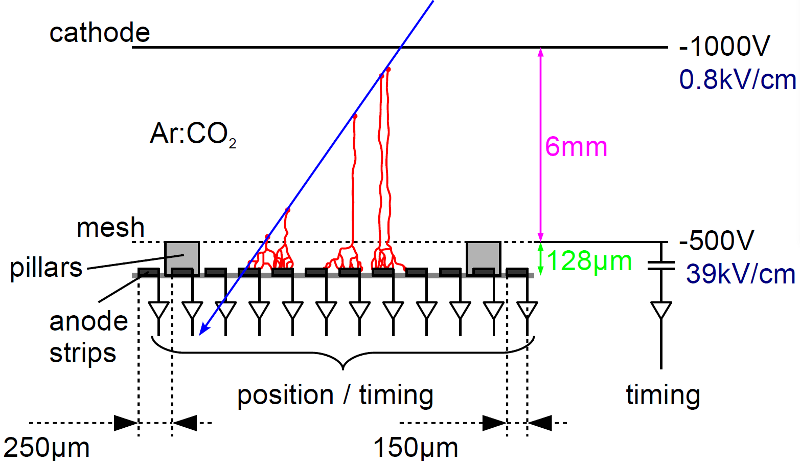
\includegraphics[width=\linewidth]{figures/detector_readout.png}
  \caption{setup of micromegas detector with a two dimensional readout}
  \label{fig:readout}
\end{figure}

\subsection{Mutiplie scattering}\label{subsec:theory_scattering}
When a charged particle travels through a material, it undergoes numerous interactions with the nucleus. Each interaction causes a small angular deflection due to the electric field of the nucleus. The result of these many angle deflections is known as multiple scattering. As the particle travels through the medium, these deflections add up. The distribution of the resulting deflection angles is approximately Gaussian in the central region. This statistical treatment of deflections allows us to describe the angular distribution with a root mean square (RMS) scattering angle.
A used formula to estimate the RMS projected scattering angle is given by the Highland approximation. The Highland formula is expressed as
\begin{equation}\label{eq:Highland}
    \theta_0 = \frac{13.6\,\text{MeV}}{\beta cp} \, z \, \sqrt{\frac{x}{X_0}} \left[1 + 0.038 \ln\left(\frac{x}{X_0}\right)\right],
\end{equation}
where $\theta_0$ is the RMS scattering angle in the projected plane, $p$ is the momentum of the incident particle, $\beta$ is its velocity divided by the speed of light, $z$ is the charge number of the particle, $x$ is the thickness of the target material, and $X_0$ is the radiation length of the material.

The angular distribution of scattered particles, in the small-angle approximation, follows a Gaussian probability distribution centered around the initial direction of the particle beam:
\begin{equation}\label{eq:Gauss}
P(\theta) = \frac{1}{\sqrt{2\pi} \, \theta_0} \exp\left( -\frac{\theta^2}{2\theta_0^2} \right).
\end{equation}
In experimental setups, the angular spread caused by multiple scattering can be observed by placing a detector at a known distance $d$ from the target. The scattered beam appears will result broadened results of the detector plots, and the standard deviation $\sigma$ of this lateral beam profile is related to the angular RMS via simple geometric considerations. Specifically, the relation
\begin{equation}\label{eq:sigma}
    \sigma = d \cdot \theta_0
\end{equation}
connects the physical spread of the beam. From this, the angular spread can be experimentally inferred using the expression
\begin{equation}\label{eq:theta_exp}
\theta_{\text{exp}} = \arctan\left( \frac{\sigma}{d} \right).
\end{equation}
for small deflection angles. Important to the Gaussian is that the shape and width of the Gaussian angular distribution are sensitive to several physical parameters. Increasing the distance $d$ between the target and the detector results in a proportional increase in the lateral spread in  \autoref{eq:sigma} making the distribution appear wider.
Changing the thickness $x$ of the target material has a direct impact. Since the RMS angle $\theta_0$ grows with $\sqrt{x}$, a thicker leads to broader angular distributions due to more scattering events. Likewise, decreasing the radiation length $X_0$ increases $\theta_0$, again broadening the Gaussian spread. Therefore, materials with shorter radiation lengths cause more significant angular deflection over the same thickness.
Since $\theta_0$ scales linearly with $z$, particles with higher electric charge will scatter more strongly. This results in a wider Gaussian distribution.

%-----------------------------------------------------------------------------------------------------------------------------

\section{Cosmic Data}
\subsection{Measuring of Detector Specifications} \label{subsec:detector_specific} % structure? 
For a deeper understanding of the structure of a micromegas detector the spare detector depicted in \autoref{fig:micromegas_closed} was disassambled.
While disassambling the detector we measured some specifications of the given device.

\begin{figure}
  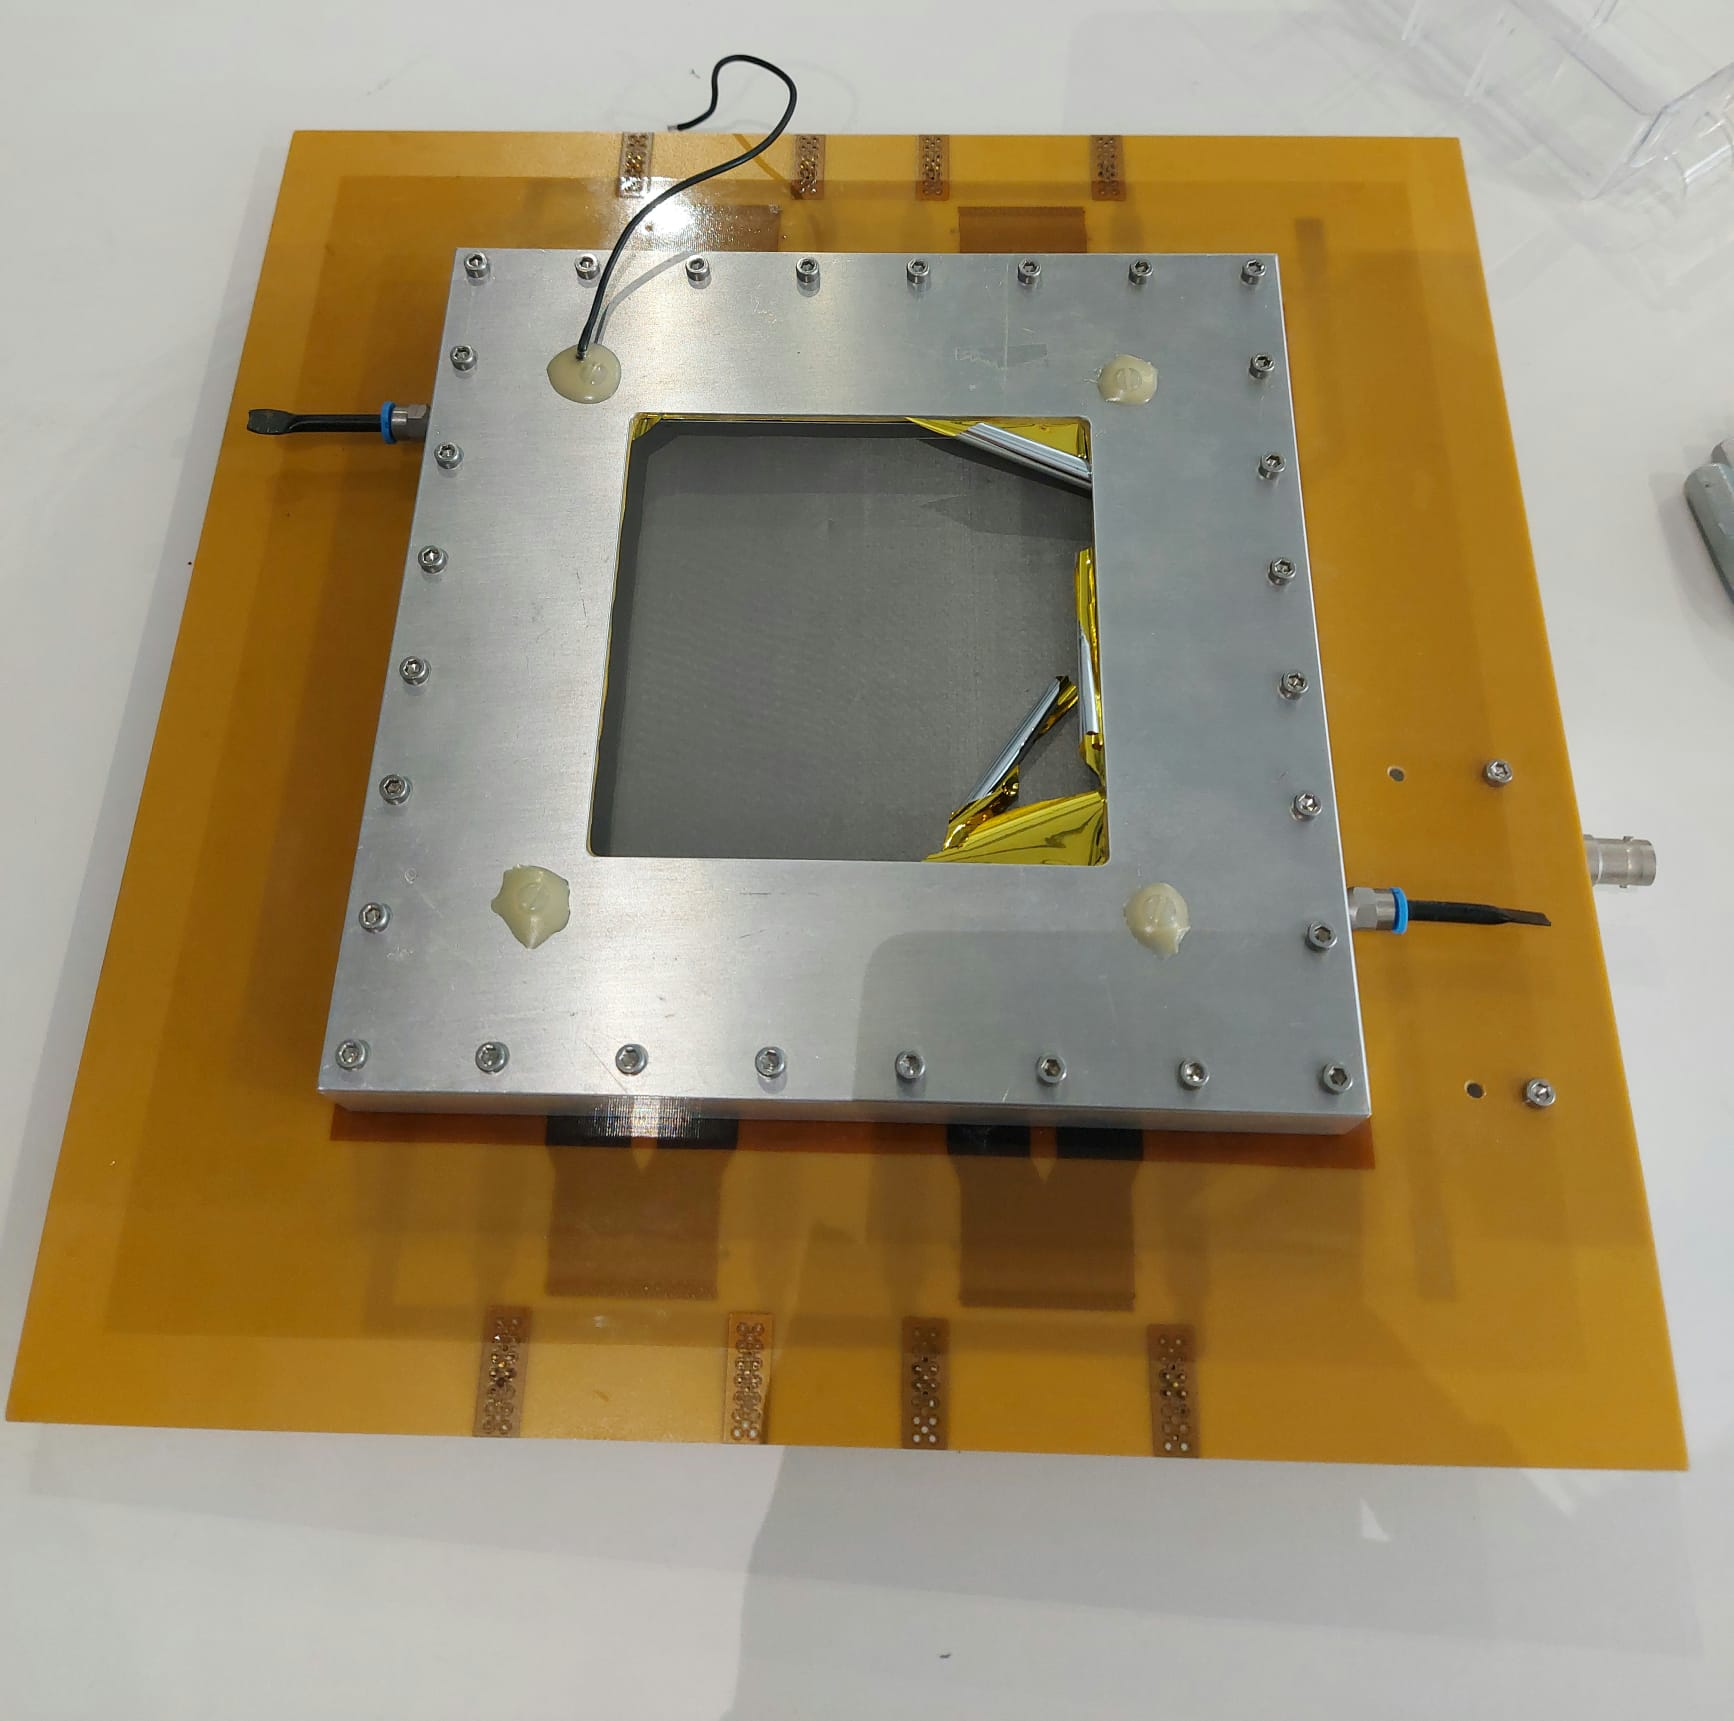
\includegraphics[width=\linewidth]{figures/micromegas_closed.jpeg}
  \caption{Front of the spare micromegas detector}
  \label{fig:micromegas_closed}
\end{figure}

To access the inner part of the micromegas detector the screws on the top need to be removed.
After that the upper part is removed. Attached to the upper metal part is a mesh which is held by four plasic pillars as can be seen in \autoref{fig:micromegas_cover}.
This mesh is functioning as the cathode of our detector. We measured the distance between the entry window and the cathode to be \SI{1.0\pm.2}{\centi\meter} aswell as the diameter of the cathode to be \SI{11\pm.2}{\centi\meter}.
Our measurements were done with the help of a lineal and we therefore assumed an uncertaincy of \SI{.2}{\centi\meter} on all measurements.

\begin{figure}
  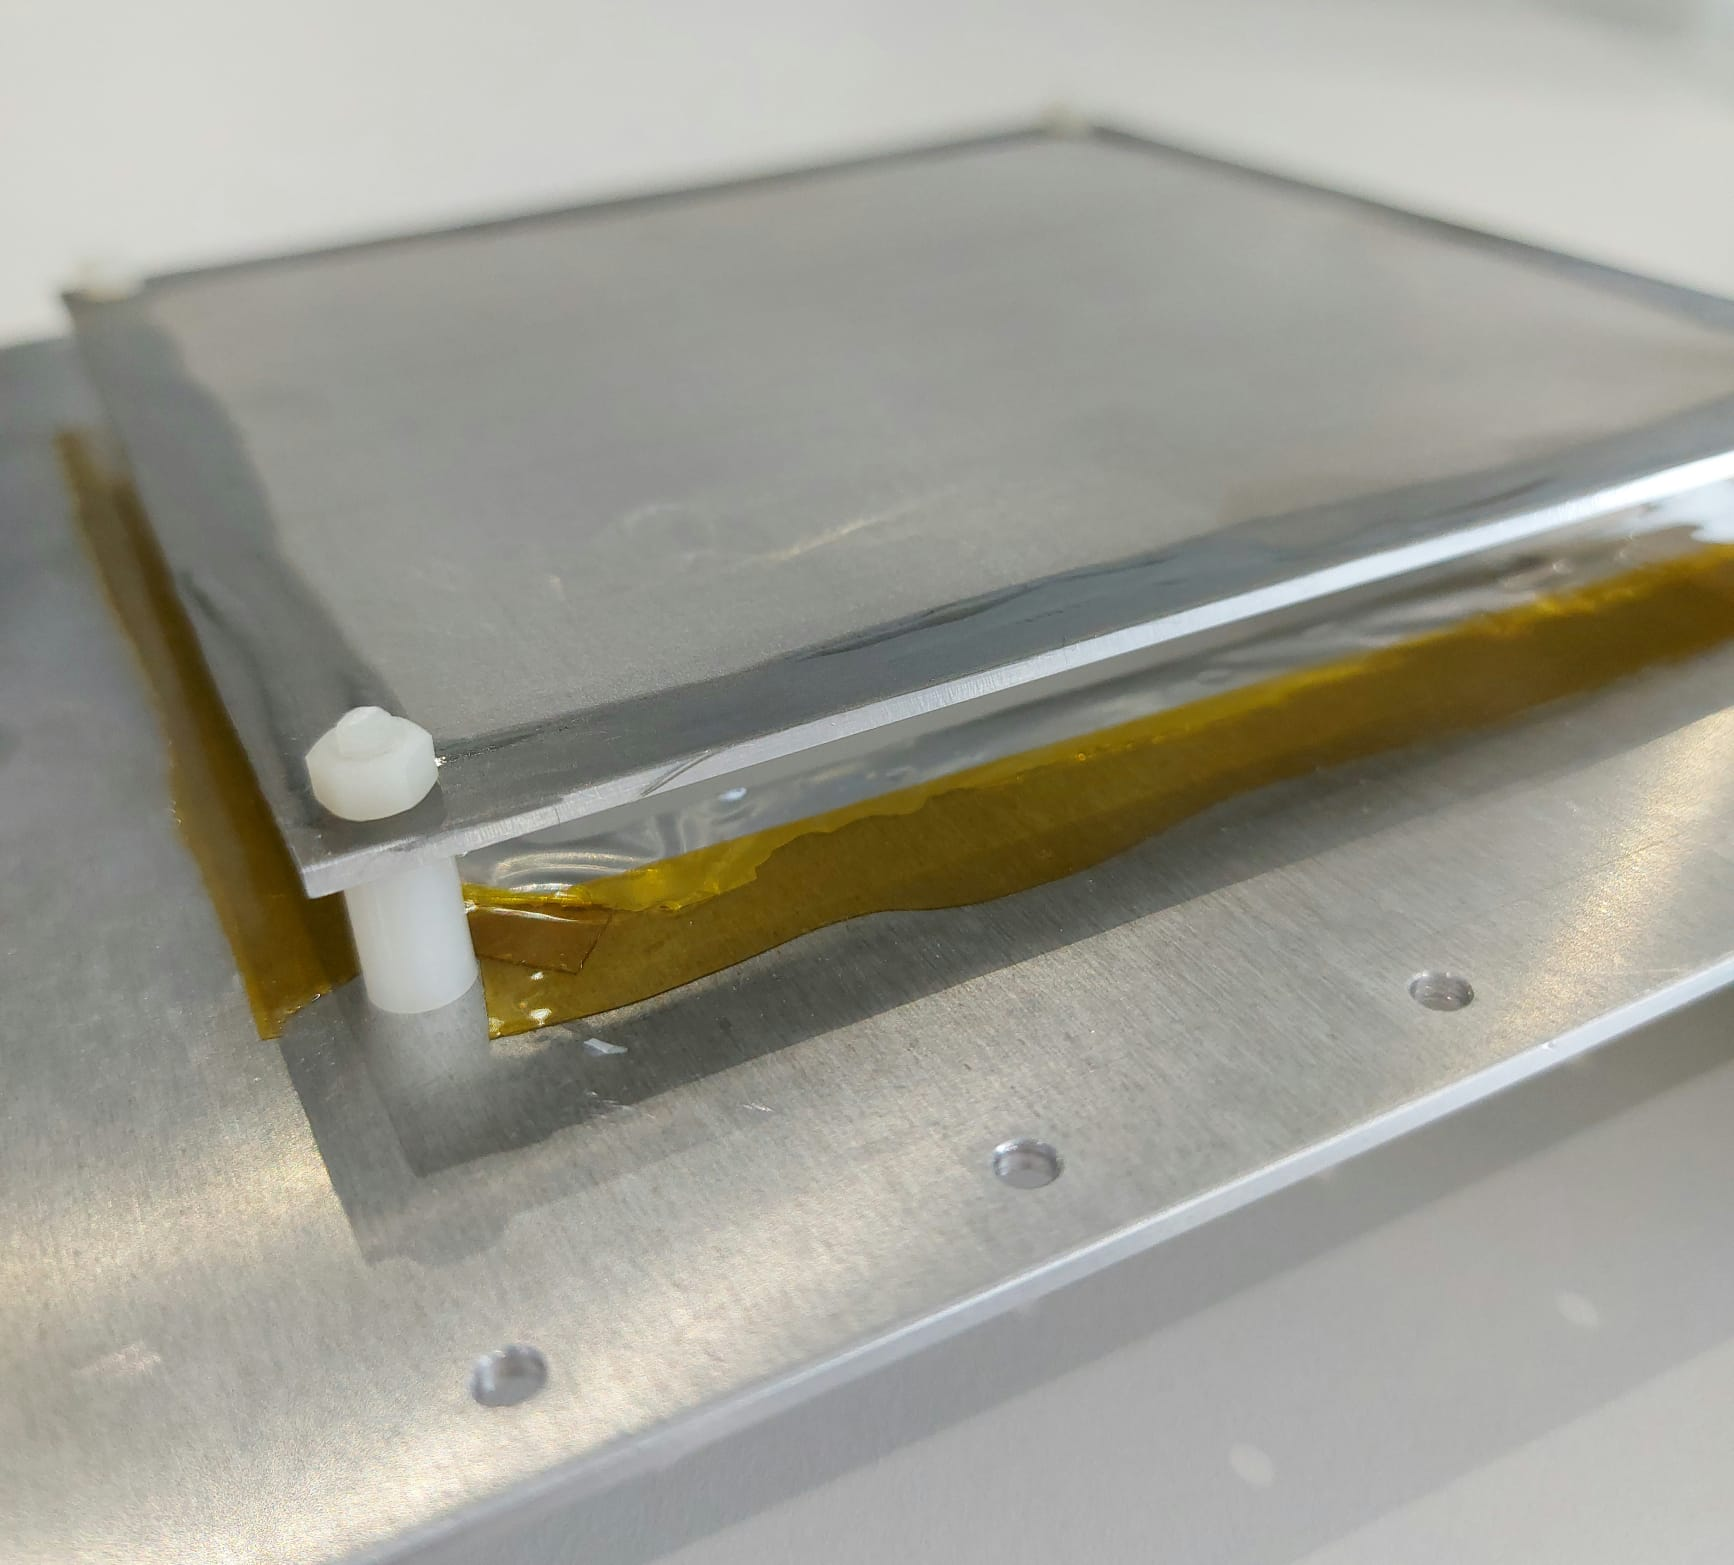
\includegraphics[width=\linewidth]{figures/micromegas_cover.jpeg}
  \caption{Mesh on the upper part of the micromegas}
  \label{fig:micromegas_cover}
\end{figure}

More interesting is not the cover of the micromegas but what lies underneath.
In \autoref{fig:micromegas_base} we can see the inside of our detector. The cathode was placed in the center gap.
At the bottom we can see the mesh of the detector, which is responsible for gasamplification like explained in \autoref{subsec:theory_micromegas}.
We measured the inner diameter of the mesh to be \SI{13.8\pm.2}{\centi\meter}.

\begin{figure}
  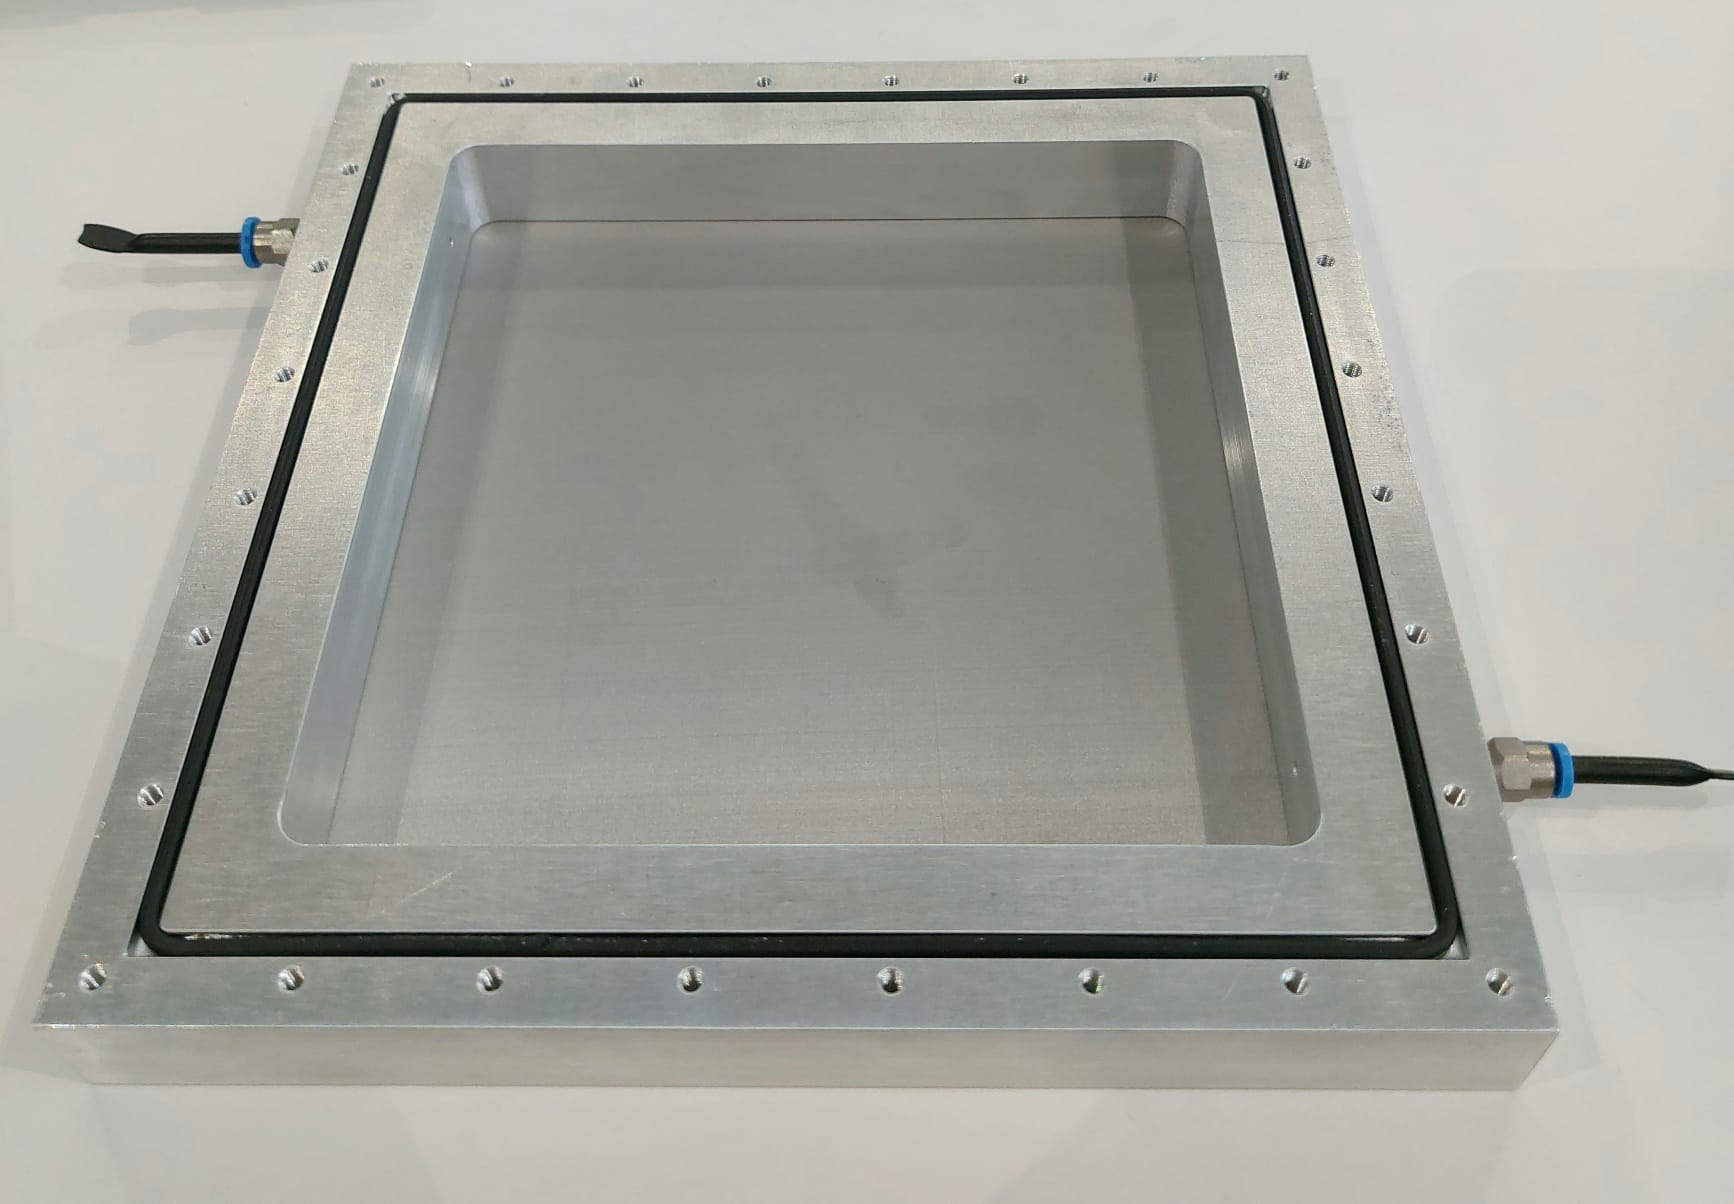
\includegraphics[width=\linewidth]{figures/micromegas_base_top.jpeg}
  \caption{Bottom part of the micromegas with the mesh}
  \label{fig:micromegas_base}
\end{figure}

Below the mesh one can see the anode strips on the PCB wafer shown in \autoref{fig:micromegas_strips}.
We measured the activ area, so the area covered with anodes, to be \SI{10\pm2.8}{\cm^2} where the uncertainty is calculated by the gaussian propagation of uncertainty.
One could observe a grid-like structure of the anodes. 
We measured width and height of one rectangle in this grid structure to be $\SI{4\pm1}{\mm}\times\SI{5\pm1}{\mm}$.
By further inspection we noticed that one rectangle in this structure is connected with 10 wires.
This indicates that there are 10 strips per rectangle.
Therefore we concluded that the true dimensions of one strip can be calculated as in \autoref{eq:dimensions}.
\begin{equation}\label{eq:dimensions}
  \frac{\SI{4\pm1}{\mm}\times\SI{5\pm1}{\mm}}{10}=\SI{400\pm100}{\micro\meter}\times\SI{500\pm100}{\micro\meter}  
\end{equation}

\begin{figure}
  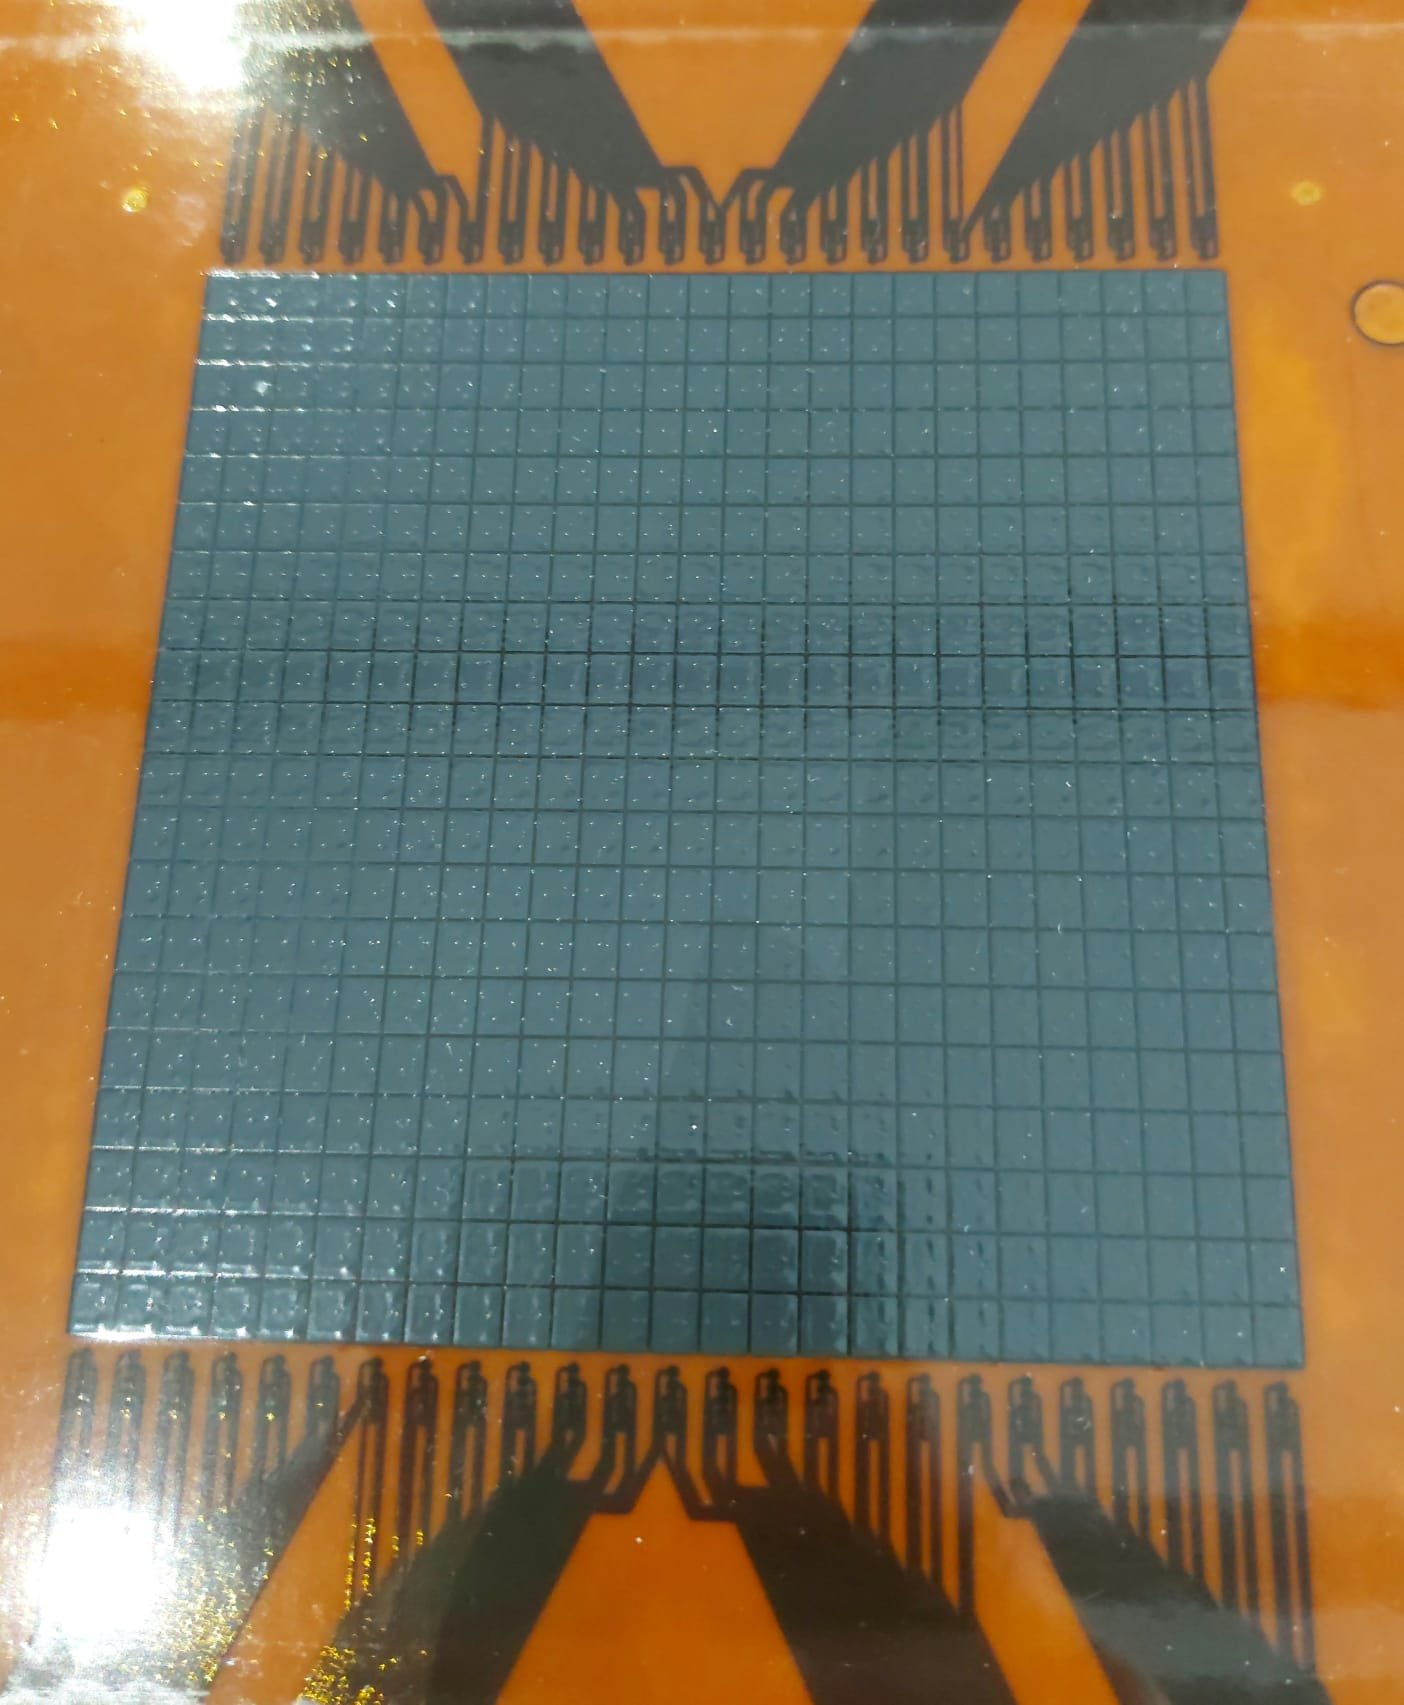
\includegraphics[width=\linewidth]{figures/micromegas_strips.jpeg}
  \caption{Grid-like structure of the anode strips}
  \label{fig:micromegas_strips}
\end{figure}

\subsection{Experimental Setup}
To observe cosmic muon rays, a micromegas detector was setup horizontally between two scintillators.
These scintillators are overlapping and positioned like shown in \autoref{fig:setup_ROT}.

\begin{figure}
  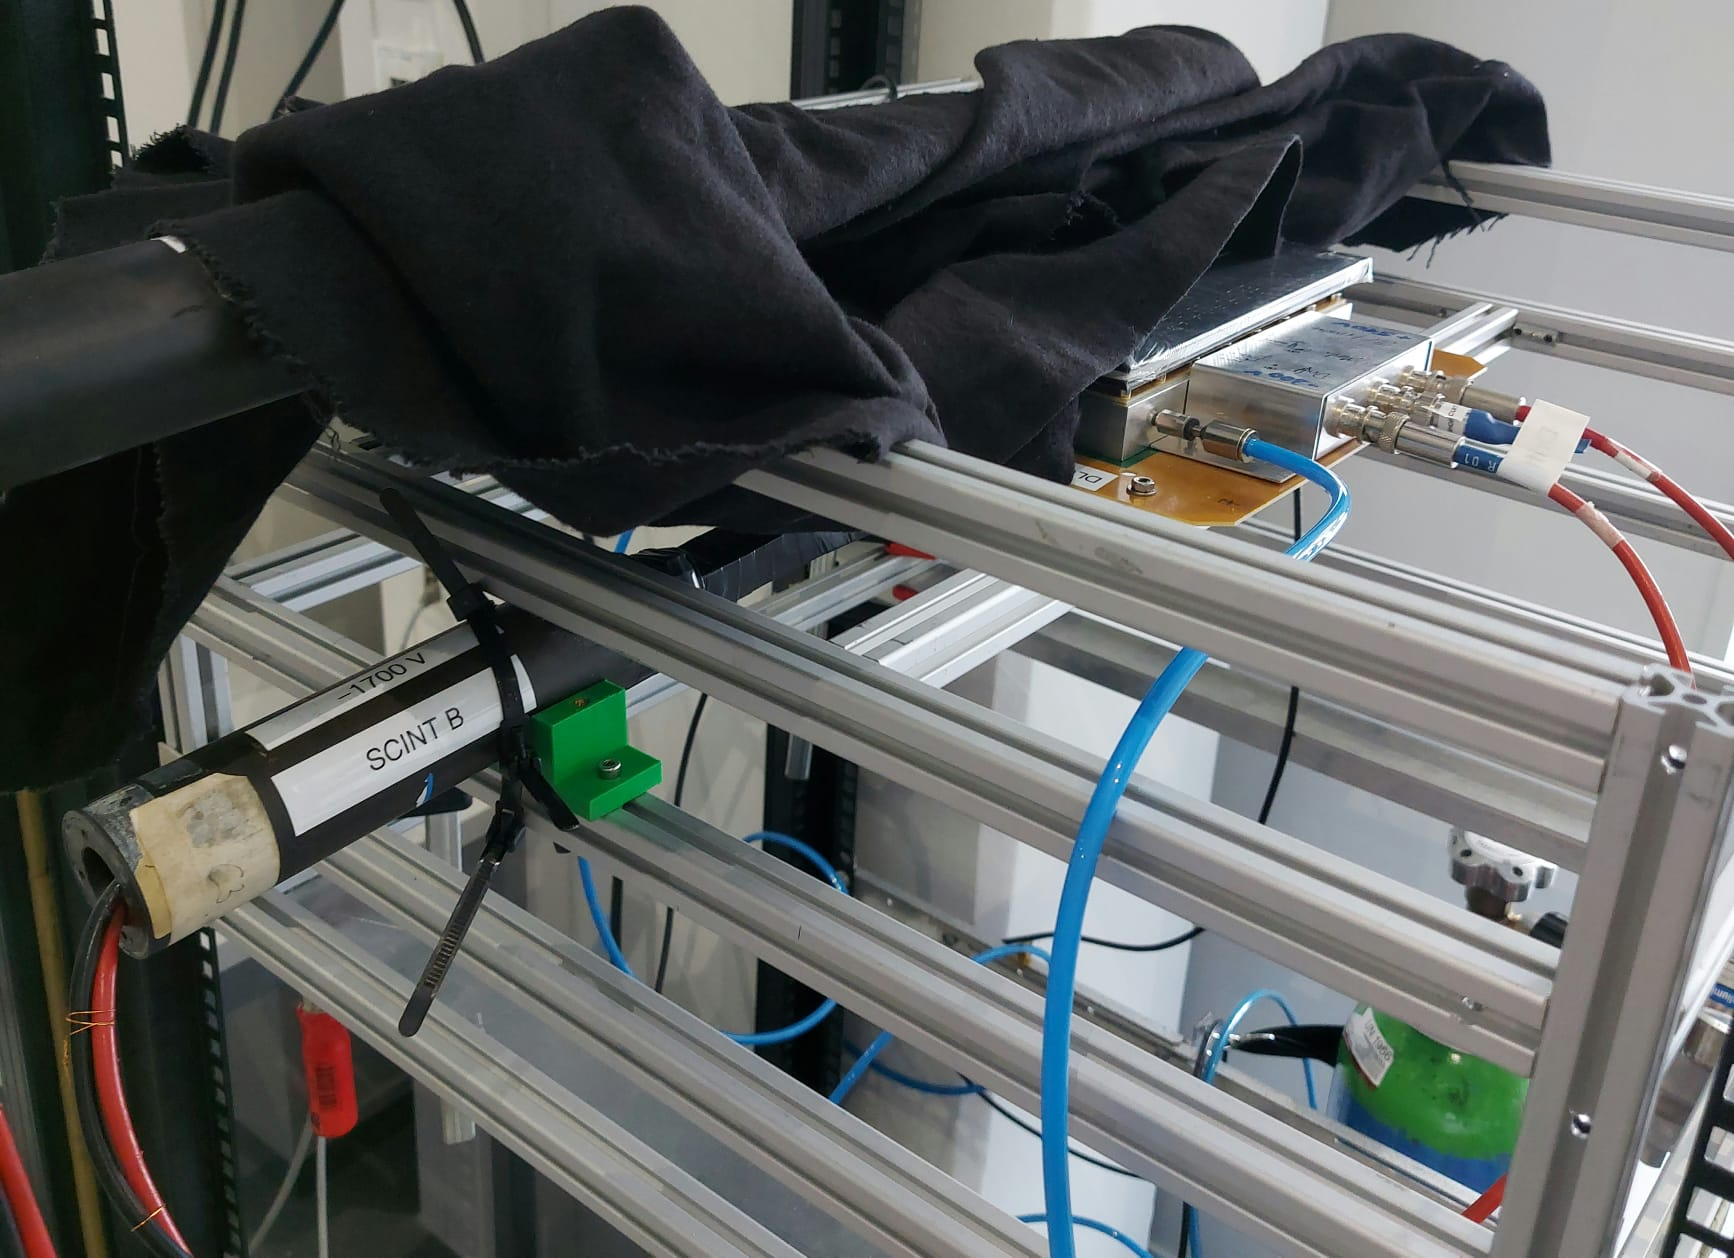
\includegraphics[width=\linewidth]{figures/setup_ROT.jpeg}
  \caption{Used setup of micromegas detector and scintillators at ROT to measure cosmic muon events}
  \label{fig:setup_ROT}
\end{figure}

As can be seen, one of the scintillators is covered up by a cloth. This is because a previous group noticed that this particular scintillator did not seem to be sealed correctely and thus covered it to increase its efficiency.
The scintillators are provided with voltages of \SI{1700}{\volt} and \SI{1250}{\volt}. These voltages along with the voltages for the micromegas detector of \SI{-300}{\volt} and \SI{510}{\volt} are provided by a high voltage module.
Additionally to the high voltage module more modules are used to set up the trigger logic of the detector.
The trigger logic ensures, that the detector only counts events when both scintillators register an event so noise is minimized and only particles which pass through the detector are counted.
The readout system of the detector consists of four APVs and a minicrate, which are triggered by the trigger logic and send the received data to a PC where the data readout is handeled by the DAQ software.
(...) % explanation and handling of DAQ? 

\subsection{Experimental Procedure}
To set up the trigger logic we first put the scintillators directly on top of each other, so events would be registered at both of them at a higher rate.
This positioning was only used in first setting up the trigger logic.
For data taking we returned the scintillators to their original positions above and below the micromegas detector.
Looking at the scintillator signal directly with an oscilloscope we could obseve a signal like shown in \autoref{fig:scintillator_signal}.

\begin{figure}
  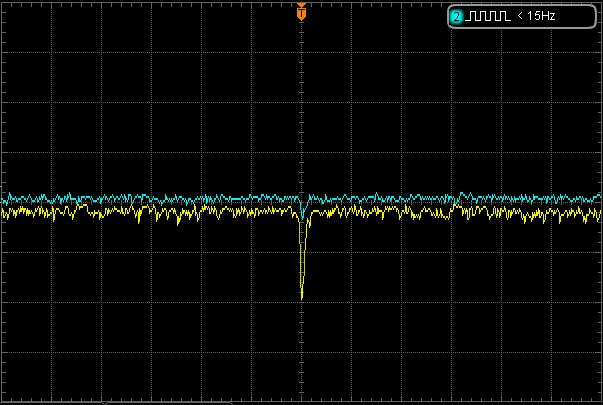
\includegraphics[width=\linewidth]{figures/DS1Z_QuickPrint5_cropped.png}
  \caption{Signal of both scintillators without modification}
  \label{fig:scintillator_signal}
\end{figure}

The signals are quite weak, so we first amplified them using the 12-channel photomultiplier amplifier module which has a gain of 10.
After amplifying the signal we want to discriminate it, so we can more easily look for coincidence of both scintillator signals.
The discriminator only triggeres when a certain signal threshold is reached like depicted in \autoref{fig:discriminator}. 
When triggered the discriminator outputs a signal over a given discrimination time.
By setting the threshold we can filter out most of the noise.
Because the discriminator has a set discrimination time multilpe events in this time will not be registered. 
For measuring cosmic muon rays this is not relevant because the events are of low enough frequency.

\begin{figure}
  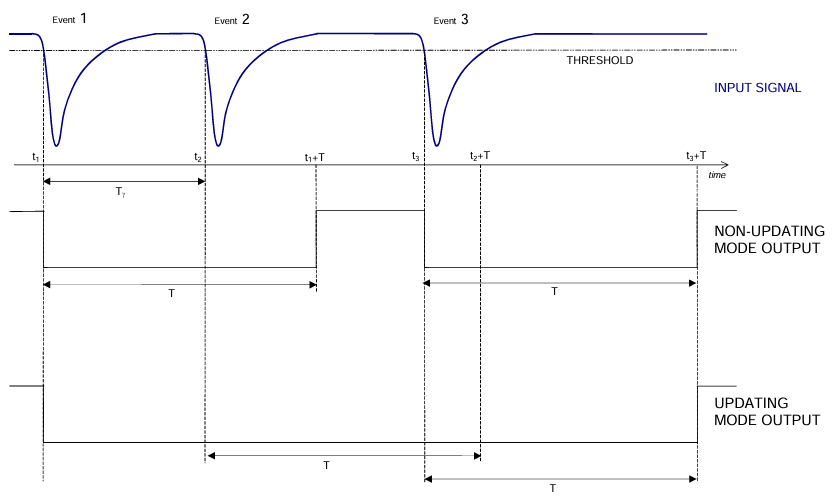
\includegraphics[width=\linewidth]{figures/discriminator.png}
  \caption{Working principle of the Mod. N841 16 Channel Leading Edge Discriminator}
  \label{fig:discriminator}
\end{figure}

After we produced the discriminated signal we want to check for coincidence between both signals of the scintillators.
To achieve this we use a logic unit with an \textsc{and} operation on both discriminated signals.
This yields only a signal when both scintillators have overlapping discrimination signals like shown in \autoref{fig:disc_signal}.
Because of the overlap it can be assumed that both scintillator signals stem from the same particle passing though them.
When there is no overlap we assume that the scintillators are hit by different particles and we get no trigger signal.
At last we count the registered events with a simple counter module to check if our trigger is registering events at a realistic rate.
Now we have finished our trigger logic and we only trigger the detector readout when both scintillators register an overlapping signal.
This means that a particle has hit both of the scintillators and thus has passed through our micromegas detector.

\begin{figure}
  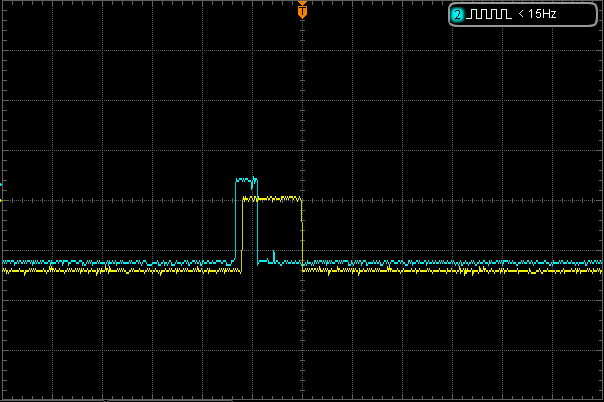
\includegraphics[width=\linewidth]{figures/DS1Z_QuickPrint2_cropped.png}
  \caption{Discriminated signal of one scintillator (yellow) and trigger signal after logic unit (blue)}
  \label{fig:disc_signal}
\end{figure}

After setting up the trigger logic we are ready to take data. First we need to take a pedestal run in the DAQ to configure the readout electronics.
When the pedestal run is finished the real data taking can start. 
We took data over a time of roughly \SI{30}{\minute} and then extracted the informations from the root file which yields the hitmap in \autoref{fig:muon_hitmap}. (???) % time correct?

% why averaged, and how exactly?
\begin{figure}
  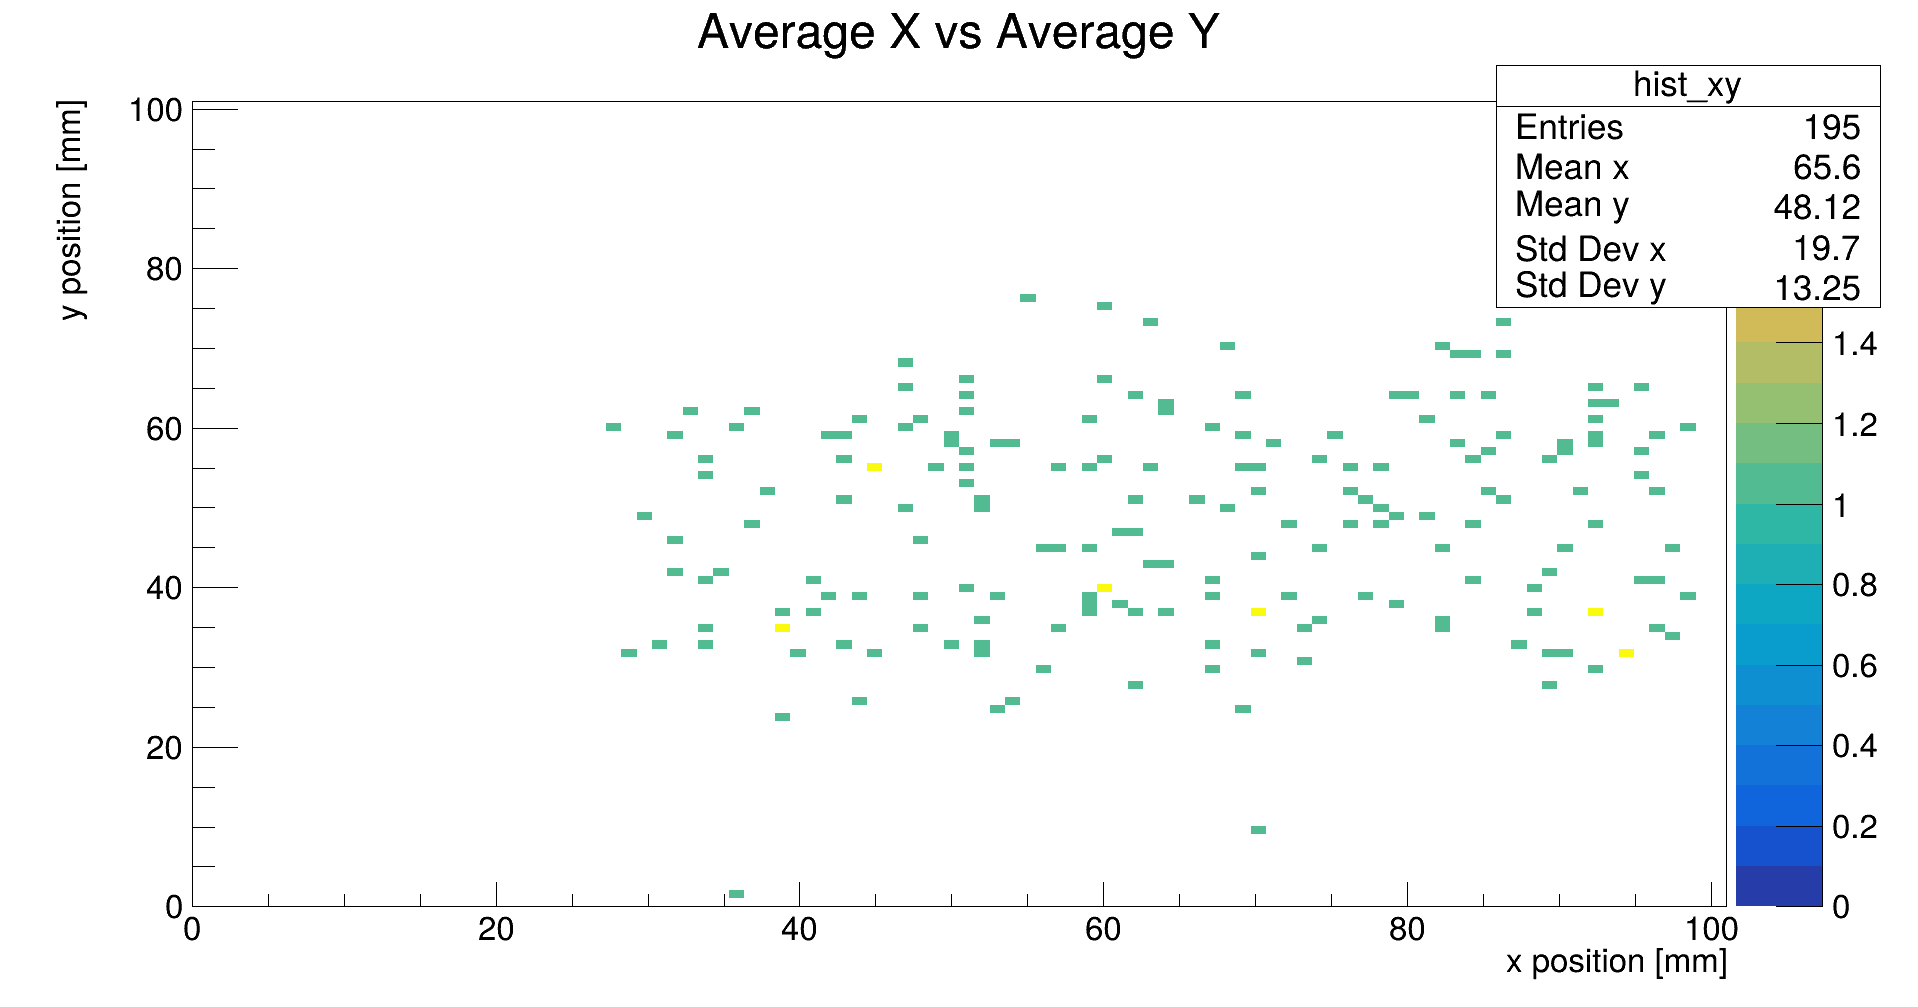
\includegraphics[width=\linewidth]{../src/elsa/finished_plots/muon_hitmap_avg.png}
  \caption{Averaged hitmap of cosmic muons}
  \label{fig:muon_hitmap}
\end{figure}

As can be seen our scintillators were orientated parallel to each other and overlapped along their whole length.
Because of our trigger logic we only register events at places where our scintillators overlap. 
It is clear that other events may have happened but were not read out because our trigger logic did not register overlapping scintillator signals.
The muons seem to be evenly distributed over the area of the scintillators which seems logical, because cosmic radiation should be homogeneously distributed.
We can also see some events which are not in the area of our scintillators. 
Those can either be explained by noise or other interferences in the data taking process.
It can also be possible that the detector readout was triggered by an event in the area of the scintillators while another event happened at a different place in the detector.
Because one event triggered the detector readout another event which happened may have been read out as well.
(???)

% Questions:
% picture of modules after setting up trigger logic?
% working principle of scintillators? 
% description of readout system and DAQ?

%-----------------------------------------------------------------------------------------------------------------------------

\section{Multiple Scattering}
\subsection{Experimental Setup}
To observe multiple scattering, a electron beam of $\SI{2.9}{GeV}$ is provided by the stretcher ring of ELSA, whose exit is shown in \autoref{fig:beam_setup_elsa}. The setup of the micromegas detector with the scintillators and the trigger logic, used and tested with the cosmic data, is placed a few meters in front of the output of the accelerator, such that the beam hits the detector as seen in \autoref{fig:detector_setup_elsa}. This is ensured by a laser, build in at the end of the accelerator, which could be slid into the middle of the opening to point along the beam line. However, it is known that the laser points a few centimeters too low compared to the actual beam. This must be note by constructing the setup and while placing the targets.
To do latter, a metal bar is mounted close to the detector thus the targets could be placed in a distance between $\SI{5.5\pm 0.5}{cm}$ and $\SI{105.5\pm 0.5}{cm}$ to the first scintillator into the beam, where the uncertainties come from the measuring tape used to evaluate these distances. Thereby, the laser is used to adjust the bar and to ensure a free beam path up to the detector or the placed material.
The available materials with their thicknesses are listed in \autoref{tab:available_materials}. These were measured by a previous group with a caliper, so uncertainties of $\SI{0.1}{mm}$ are assumed, which is roughly checked with the maesuring tape.


\begin{table}\centering
  \renewcommand*{\arraystretch}{1.1}
  \begin{tabular}{c|c||c|c}
    \multicolumn{2}{c||}{Aluminum} & \multicolumn{2}{c}{Copper} \\
    {\fontsize{8}{3}\selectfont $d/\si{cm}$} & {\fontsize{8}{3}\selectfont \#} & {\fontsize{8}{3}\selectfont $d/\si{cm}$} & {\fontsize{8}{3}\selectfont \# } \\\hline \rule{0pt}{3ex}
    \num{1.22\pm 0.01} & 2 & \num{0.2\pm 0.01} & 3 \\
    \num{2.5\pm 0.01} & 1 & \num{0.5\pm 0.01} & 2 \\
    \num{5\pm 0.01} & 1 & \num{1.48\pm 0.01} & 2 \\
    \num{9.96\pm 0.01} & 1 & & \\
    \num{9.93\pm 0.01} & 1 & & \\
  \end{tabular}\vspace{3mm}
  \caption{Available scattering materials of thickness $d$ and quantity $\#$.}
  \label{tab:available_materials}
\end{table}

\begin{figure}
  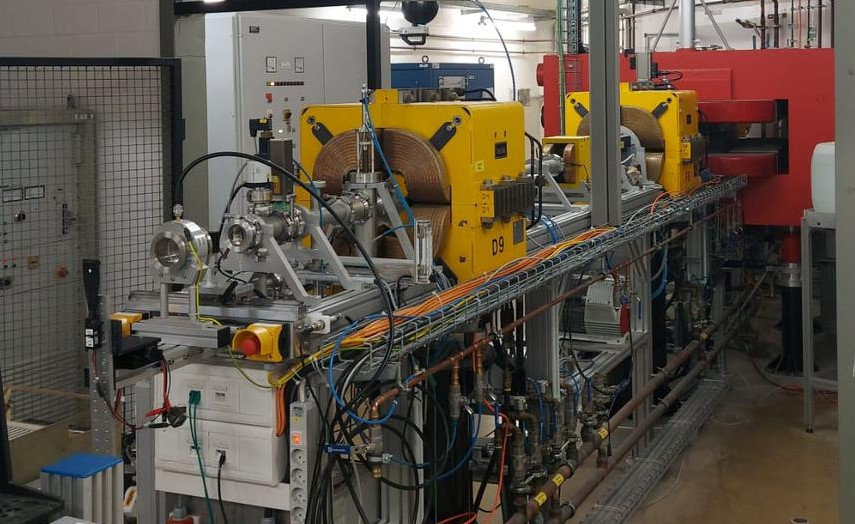
\includegraphics[width=\linewidth]{figures/beam_setup_elsa.jpg}
  \caption{Exit of ELSA.}
  \label{fig:beam_setup_elsa}
\end{figure}

\begin{figure}
  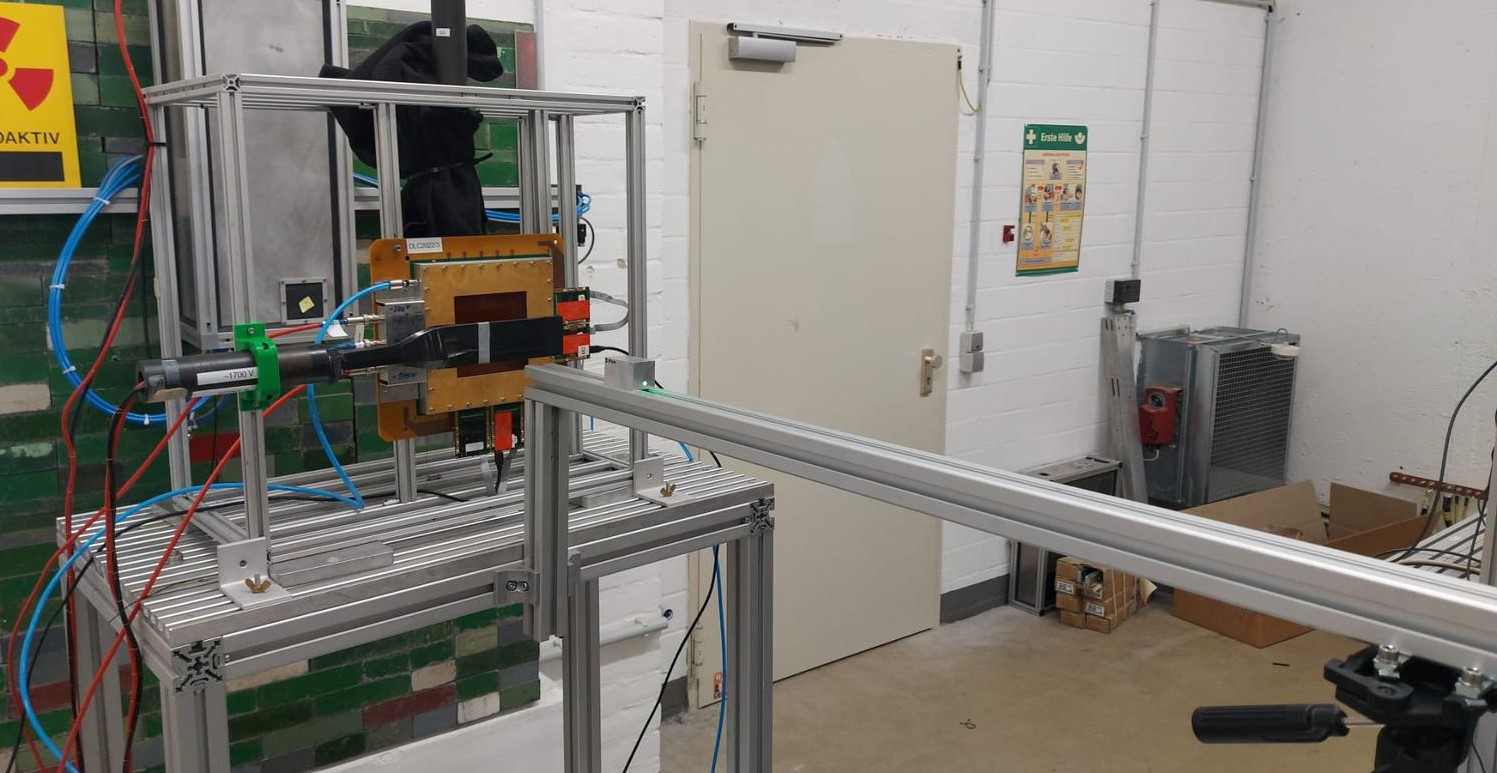
\includegraphics[width=\linewidth]{figures/detector_setup_elsa.jpg}
  \caption{Setup of the detector and the metal bar, to place the targets on it and align them with the laser.}
  \label{fig:detector_setup_elsa}
\end{figure}

\subsection{Experimental Procedure}
After controlling the setup of the detector including the trigger logic and the right adjustment of the metal bar, a test run without any target in the beam is performed, to ensure the functionality of the setup and the data taking program DAQ.
Afterwards, for both materials multiple runs are recorded. Thereby, the thicknesses $D$ of the targets are changed by placing different blocks of one material in a row. $D$ is approximately always chosen to be different multiples $m$ of the radiation length $X_0$ of the material, with $m\in\{0.5,1,2,3\}$. The distance $z$ between the scintillator and the leading edge of the material is always $z=\SI{40\pm0.5}{cm}$. Overall eight runs, one for each $m$ and both materials, are recorded. The exact configurations for the different recordings are listed in \autoref{tab:config_materials}.

\begin{table}\centering
  \renewcommand*{\arraystretch}{1.15}
  \begin{tabular}{c|c|c}
    & Aluminum & Copper \\
    & {\fontsize{7}{5}\selectfont ($X_0=\SI{8.897}{cm}$)} & {\fontsize{7}{5}\selectfont ($X_0=\SI{1.436}{cm}$)} \\\hline
    $m$ & $\sum d/cm = D /cm$ & $\sum d/cm = D /cm$ \\\hline\hline\rule{0pt}{6ex}
    $0.5$ & \num{5\pm 0.01} & $\begin{array}{r}
                \num{0.5\pm 0.01} \\
                +\,\num{0.2\pm 0.01} \\\hline
                =\,\num{0.7\pm 0.01}    
              \end{array}$ \\\hline
    $1$ & \num{9.93\pm 0.01} & \num{1.48\pm 0.01} \\\hline
    $2$ & $\begin{array}{r}
      \num{1.22\pm 0.01} \\
      +\,\num{2.5\pm 0.01} \\
      +\,\num{5\pm 0.01} \\
      +\,\num{9.93\pm 0.01} \\\hline
      =\,\num{18.65\pm 0.02}
    \end{array}$ & $\begin{array}{r}
                      2\times\num{1.48\pm 0.01} \\\hline
                      =\,\num{2.96\pm 0.01}
                    \end{array}$ \\\hline
    $3$ & $\begin{array}{r}
      \num{2.5\pm 0.01} \\
      +\,\num{5\pm 0.01} \\
      +\,\num{9.93\pm 0.01} \\
      +\,\num{9.96\pm 0.01} \\\hline
      =\,\num{27.39\pm 0.02}
    \end{array}$ & $\begin{array}{r}
                      2\times\num{0.2\pm 0.01} \\
                      +\,2\times\num{0.5\pm 0.01} \\
                      +\,2\times\num{1.48\pm 0.01} \\\hline
                      =\,\num{4.36\pm 0.02}
                    \end{array}$ \\\hline
  \end{tabular}\vspace{3mm}
  \caption{Specific configurations of used materials with radiation length $X_0$ and overall thicknesses $D$ for different multiples $m$ of $X_0$.}
  \label{tab:config_materials}
\end{table}

\subsection{Data Analysis}
The recorded data of the run without scattering material in the beam is shown as a hitmap in \autoref{fig:hitmap_notarget}. The distribution of the electrons in the x-direction is wider as in y-direction, resulting in an oval-shaped beam.
To analyse the influence of a material in order to observe multiple scattering effects, a narrower beam width is advantageous, as the additional broadening due to scattering becomes more distinguishable. Moreover, \autoref{fig:x_hist_notarget} shows, that one APV of the detector positioned in x-direction contains multiple defect stips in the region of interest. Therefore, in the following analysis, only the y-direction is considered.

The collected raw data counts unwanted hits because of different reasons. First of all, there is a noise on the detector, which is also read out when the scintillators trigger the system. To filter the noise a charge threshold is used.
Another unwanted effect are created $\delta$-electrons, which also could hit the detector and lead to multiple hits for one event i.e. one readout. Moreover, the possibility of inelastic scattering of the beam electrons in the air, leading to electromagnetic or hadronic showers, exists. This also results in multiple hits for one event. To separate these effects, one counts the number of different hits or clusters, which are contiguous hits, of one event. If there are more then two clousters, the event is ignored.

The data, filtered as described, is shown for (???) in (fig-temp).
One notice, that at one specific point i.e one specific strip in the detector, no event is counted, which is observed for all runs. This indicates, that this strip do not work properly. Because the oberservation applies only for the one distinct strip, it does not effect the overall results and can be ignored.
Moreover, the number of events increase gaussian like from low to higher values of $x$ before suddenly fall close after the maximum and starts decreasing again gaussian. This behaviour is also observed for every recorded run. Because the sharp edge is localized exactly in the middle of the detector, it is evidently caused by a different behaviour of the two APVs, used for the read out of one direction. Apparently, one have a higher charge sensitive so it counts events more likely than the other one, which results in such a shifted image. In order to evaluate the effects of multiple scattering, a gaussian distribution is fittet to the data. Thereby, the behaviour of the two different curves can either be adjusted by shifting the curves manually on a equal level, or including only one side of the distribution to the fit. To do latter, the data of one APV is mirrored, while the other one is ignored. The fitted curve to this modified data can be seen for alumnium as the scattering target with a thickness of approximately two times the radiation length in \autoref{fig:2alu} and collected for all runs in \autoref{fig:alu_gaus}.

Beyond the one defect strip, which is now additional mirrored to the other side, it is noticeable, that in a very regulary pattern the gaussian distribution contains dips in the event counter. The distance between two dips is $\SI{5}{mm}$, which matches exactly the height of one rectangle of the grid structure in the detector described in \autoref{subsec:detector_specific}. This indicates the possible reason for the dips, that every $n$-th strip in one rectangle has a lower sensitivity than the others, leading to the observed effect.

The standard deviation $\sigma_\text{mat}$ of the curves, available through the parameters of the fit, leads to the scattering angle $\theta_\text{exp}$ via \autoref{eq:theta_exp}. To consider the width of the electron distribution without any scattering, the modified standard deviation
\begin{equation} \label{eq:sigma_mod}
  \sigma = \sqrt{\sigma_\text{mat}^2 + \sigma_\text{0}^2}
\end{equation}
is used, where $\sigma_\text{0}$ is the standard deviation of the distribution without any scattering material in the beam.

To compare this experimental results with the theoretical discription, $\theta_\text{exp}$ is plotted against $\theta_\text{theo} = \theta_0$ evaluated via \autoref{eq:Highland}.



\begin{figure}
  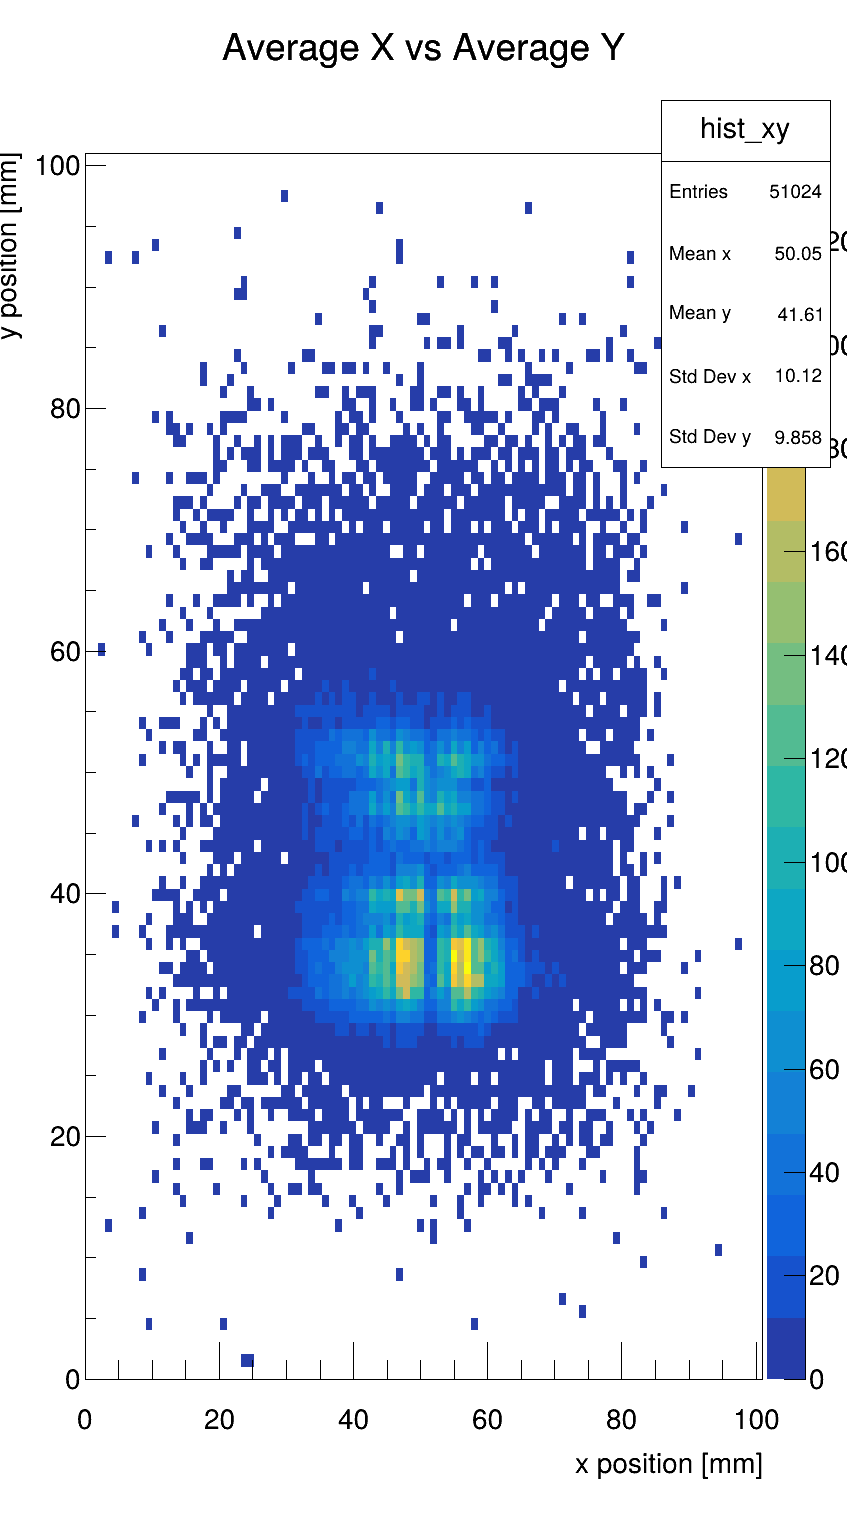
\includegraphics[width=0.9\linewidth]{../src/elsa/xy_hitmap_0.png}
  \caption{Hitmap for the electron beam on the detector without scattering material.}
  \label{fig:hitmap_notarget}
\end{figure}

\begin{figure}
  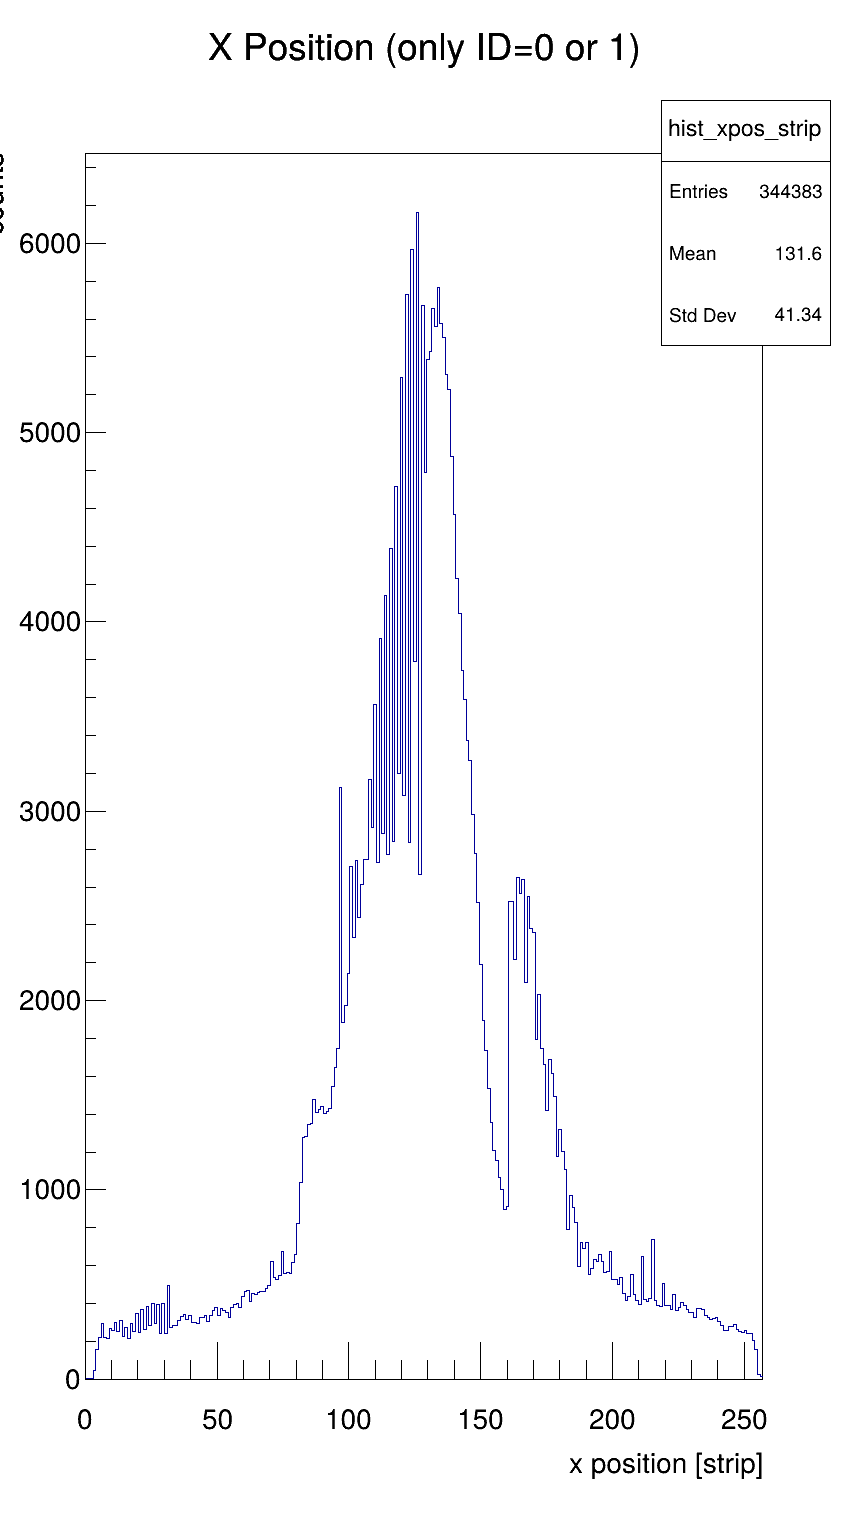
\includegraphics[width=0.9\linewidth]{../src/elsa/x_position_strip_histogram_0.png}
  \caption{Counted hits in x-direction without scattering material.}
  \label{fig:x_hist_notarget}
\end{figure}

\begin{figure}
  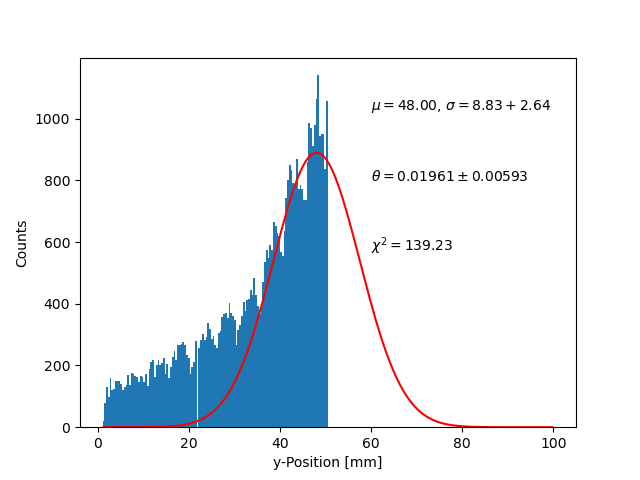
\includegraphics[width=0.9\linewidth]{../src/elsa/finished_plots/Aluminium, Two Radiation Lengths, 40cm Distance.png}
  \caption{Counted hits for alumnium with $D\approx2\cdot X_0$.}
  \label{fig:2alu}
\end{figure}







% heatmap, hitmap
% sources for X_0 
% x and y hist for no material
% explanations of each plot
% more reasons for ignoring the x data

%-----------------------------------------------------------------------------------------------------------------------------

\section{Summary}

%-----------------------------------------------------------------------------------------------------------------------------

\begin{appendices}\onecolumn

\section{Gaussian Distributions of Multiple Scattering for Ovserved Materials}

\begin{figure}[h]
    \centering
    \begin{subfigure}{0.49\textwidth}
        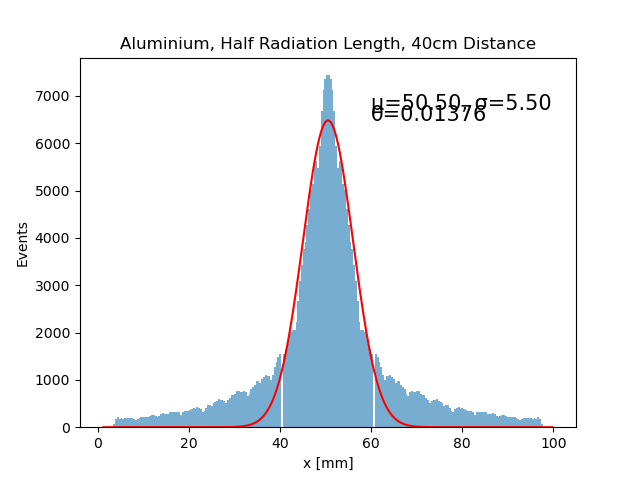
\includegraphics[width=\textwidth]{../src/elsa/finished_plots/Aluminium, Half Radiation Length, 40cm Distance.png}
        \caption{$D\approx\frac{X_0}{2}$}
    \end{subfigure}
    \begin{subfigure}{0.49\textwidth}
        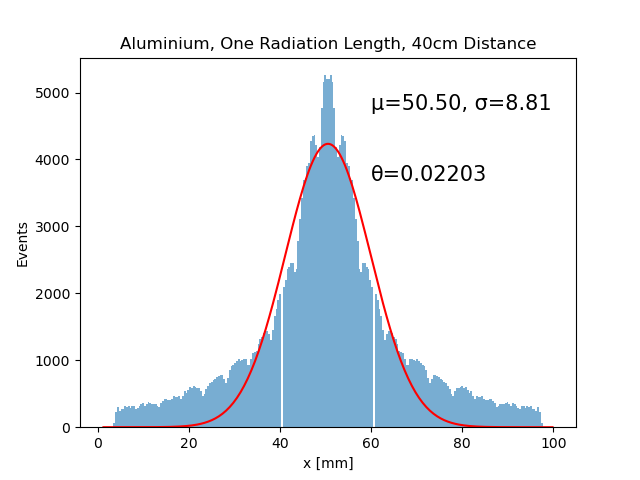
\includegraphics[width=\textwidth]{../src/elsa/finished_plots/Aluminium, One Radiation Length, 40cm Distance.png}
        \caption{$D\approx X_0$}
    \end{subfigure}
    \begin{subfigure}{0.49\textwidth}
        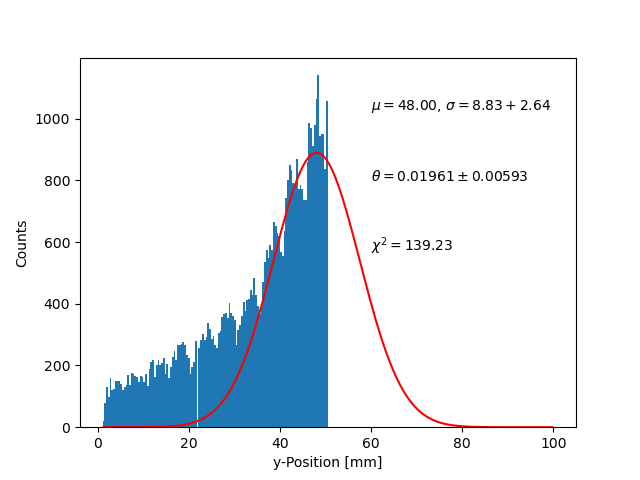
\includegraphics[width=\textwidth]{../src/elsa/finished_plots/Aluminium, Two Radiation Lengths, 40cm Distance.png}
        \caption{$D\approx2\cdot X_0$}
    \end{subfigure}
    \begin{subfigure}{0.49\textwidth}
        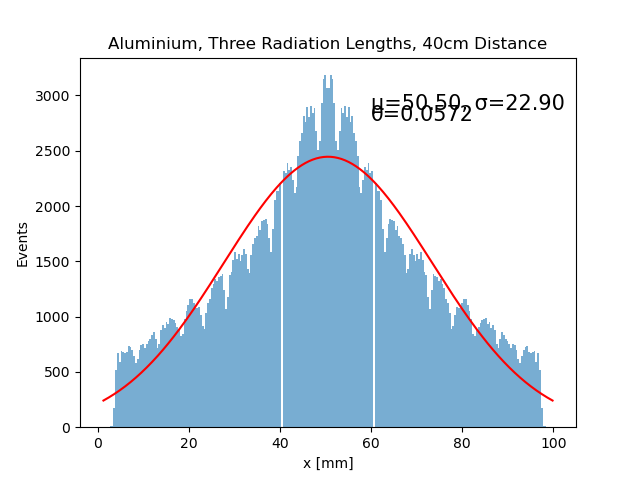
\includegraphics[width=\textwidth]{../src/elsa/finished_plots/Aluminium, Three Radiation Lengths, 40cm Distance.png}
        \caption{$D\approx3\cdot X_0$}
    \end{subfigure}
    \caption{Counted hits for alumnium of different thicknisses $D$.}
    \label{fig:alu_gaus}
\end{figure}

\begin{figure}[h]
    \centering
    \begin{subfigure}{0.49\textwidth}
        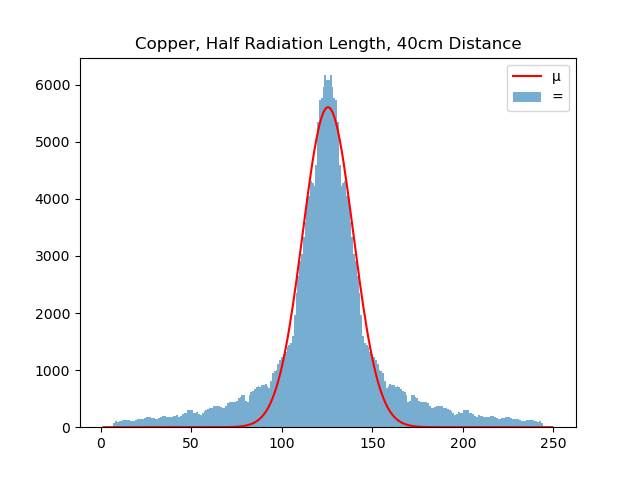
\includegraphics[width=\textwidth]{../src/elsa/finished_plots/Copper, Half Radiation Length, 40cm Distance.png}
        \caption{$D\approx\frac{X_0}{2}$}
    \end{subfigure}
    \begin{subfigure}{0.49\textwidth}
        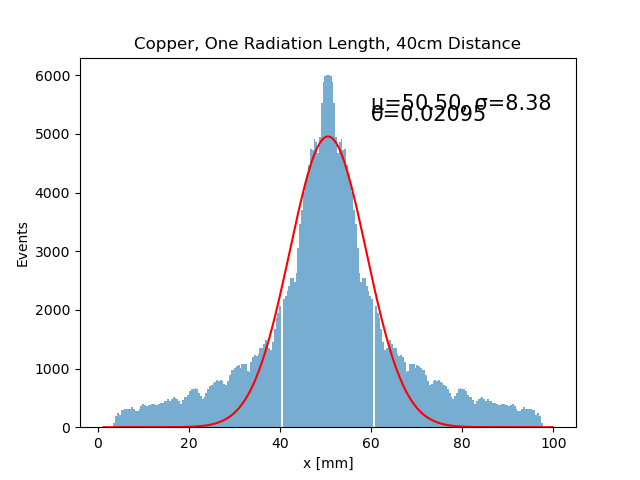
\includegraphics[width=\textwidth]{../src/elsa/finished_plots/Copper, One Radiation Length, 40cm Distance.png}
        \caption{$D\approx X_0$}
    \end{subfigure}
    \begin{subfigure}{0.49\textwidth}
        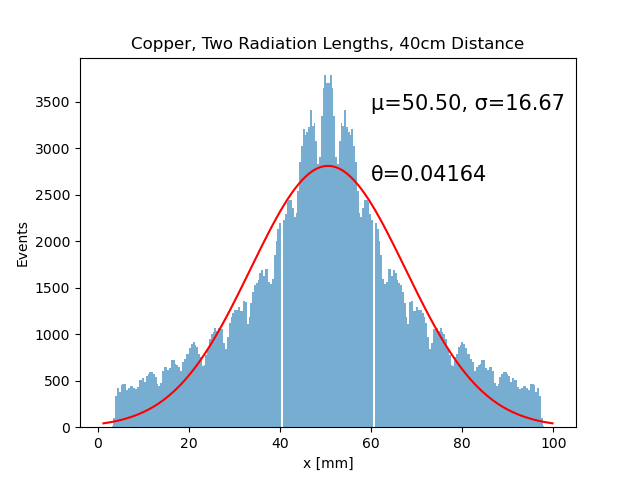
\includegraphics[width=\textwidth]{../src/elsa/finished_plots/Copper, Two Radiation Lengths, 40cm Distance.png}
        \caption{$D\approx2\cdot X_0$}
    \end{subfigure}
    \begin{subfigure}{0.49\textwidth}
        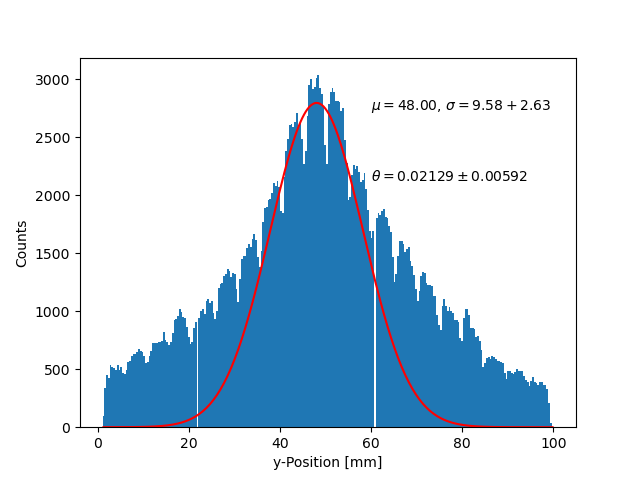
\includegraphics[width=\textwidth]{../src/elsa/finished_plots/Copper, Three Radiation Lengths, 40cm Distance.png}
        \caption{$D\approx3\cdot X_0$}
    \end{subfigure}
    \caption{Counted hits for copper of different thicknisses $D$.}
    \label{fig:cop_gaus}
\end{figure}


\end{appendices}

%-----------------------------------------------------------------------------------------------------------------------------

\clearpage
\section{Analysis ELSA (\textbf{temporary informations})}
Here is a quick rundown of how the analysis for ELSA works.

The way that the data taking works is that the detector triggers about every $\SI{25}{ns}$ and reads all strips.
It needs some time to reset and then does it again.
For ELSA data will be lost at downtime and the detector will basically trigger continuously because of the steady electron beam.

The data will be such that one event (i.e.\ one trigger) contains (most probably) multiple hits (i.e.\ multiple strips fire / register a hit).
Ideally, one would like only a single electron registered as a single hit.
This poses a problem because there are many different reasons for the undesired multiple hits.
\begin{enumerate}[label=\arabic*)]
  \item There is a certain noise on the detector, which will be registered as a hit, but this only deposits very little charge.
    To filter these events there is a certain charge threshold.
  \item It is possible, that a beam-electron creates a $\delta $-electron in the material and both hit the detector.
    This will be seen as two separate hits.
  \item The electron has a very high energy and as it traveles through the air, it is possible that it interacts with the air molecules.
    This interaction could be inelastic scattering, which would result in a Hadron shower (most likely pions) on the detector.
    This is seen (often) as a single hit (which is the electron; this hit can be very far from the expected distribution because it scattered under a higher angle) and a bunch of hits close together (Hadrons).
    To filter these events one can count the number of independent strip(s) that fired.
    Independes here means a strip or multiple strips next to each other give a signal and the adjacent strips to the left and right give none.
    These strips are called clusters.
    For example: \\\texttt{...|...||......||||..|.||.|..}\\
    would be 6 clusters.
    If the number of clusters in a single event is greater than a certain number $x$ (currently $x=2$), then this event will be left out.
\end{enumerate}
There will be a number of histograms, this includes: x and y strip events, clusters, cluster size, xy hitman etc.\

For the analysis a gaussian curve is fittet to the histogram: y strip events.
The x strips don't work well (probably detector issue and the beam has an elliptic profile).
The standard deviation of the curve is related to $\theta $ via $\tan \theta =\tfrac{\sigma }{d}$ with $d$ the distance between the target and the detector.
First calculations with this formula are in the right order of magnitude.
This will probably work better with a more precise filtering of the available data.

To evaluate the theory, $$\theta _\text{exp}=\arctan\left(\dfrac{\sigma }{d}\right)$$ is plotted against $$\theta _\text{theo}=\text{const}\,\sqrt[]{\dfrac{x}{x_0}}\left(1+0.038\ln\left(\dfrac{x}{x_0}\right)\right).$$
This should give a linear correlation between these two values thus verifying the proportionality i.e.\ the theory.
\textbf{Currently there is no correlation at all between these two so WIP.}

%\bibliography{refs}

\end{document}
